\documentclass[a4paper]{article}
\usepackage{geometry}
\usepackage{graphicx}
\usepackage{natbib}
\usepackage{amsmath}
\usepackage{amssymb}
\usepackage{amsthm}
\usepackage{paralist}
\usepackage{epstopdf}
\usepackage{tabularx}
\usepackage{longtable}
\usepackage{multirow}
\usepackage{multicol}
\usepackage[hidelinks]{hyperref}
\usepackage{fancyvrb}
\usepackage{algorithm}
\usepackage{algorithmic}
\usepackage{float}
\usepackage{paralist}
\usepackage[svgname]{xcolor}
\usepackage{enumerate}
\usepackage{array}
\usepackage{times}
\usepackage{url}
\usepackage{fancyhdr}
\usepackage{comment}
\usepackage{environ}
\usepackage{times}
\usepackage{textcomp}
\usepackage{caption}
\usepackage{multirow}


\urlstyle{rm}

\setlength\parindent{0pt} % Removes all indentation from paragraphs
\theoremstyle{definition}
\newtheorem{definition}{Definition}[]
\newtheorem{conjecture}{Conjecture}[]
\newtheorem{example}{Example}[]
\newtheorem{theorem}{Theorem}[]
\newtheorem{lemma}{Lemma}
\newtheorem{proposition}{Proposition}
\newtheorem{corollary}{Corollary}


\floatname{algorithm}{Procedure}
\renewcommand{\algorithmicrequire}{\textbf{Input:}}
\renewcommand{\algorithmicensure}{\textbf{Output:}}
\newcommand{\abs}[1]{\lvert#1\rvert}
\newcommand{\norm}[1]{\lVert#1\rVert}
\newcommand{\RR}{\mathbb{R}}
\newcommand{\CC}{\mathbb{C}}
\newcommand{\Nat}{\mathbb{N}}
\newcommand{\br}[1]{\{#1\}}
\DeclareMathOperator*{\argmin}{arg\,min}
\DeclareMathOperator*{\argmax}{arg\,max}
\renewcommand{\qedsymbol}{$\blacksquare$}

\definecolor{dkgreen}{rgb}{0,0.6,0}
\definecolor{gray}{rgb}{0.5,0.5,0.5}
\definecolor{mauve}{rgb}{0.58,0,0.82}

\newcommand{\Var}{\mathrm{Var}}
\newcommand{\Cov}{\mathrm{Cov}}

\newcommand{\vc}[1]{\boldsymbol{#1}}
\newcommand{\xv}{\vc{x}}
\newcommand{\Sigmav}{\vc{\Sigma}}
\newcommand{\alphav}{\vc{\alpha}}
\newcommand{\muv}{\vc{\mu}}

\newcommand{\red}[1]{\textcolor{red}{#1}}

\def\x{\mathbf x}
\def\y{\mathbf y}
\def\w{\mathbf w}
\def\v{\mathbf v}
\def\E{\mathbb E}
\def\V{\mathbb V}

% TO SHOW SOLUTIONS, include following (else comment out):
\newenvironment{soln}{
    \leavevmode\color{blue}\ignorespaces
}{}


\hypersetup{
%    colorlinks,
    linkcolor={red!50!black},
    citecolor={blue!50!black},
    urlcolor={blue!80!black}
}

\geometry{
  top=1in,            % <-- you want to adjust this
  inner=1in,
  outer=1in,
  bottom=1in,
  headheight=3em,       % <-- and this
  headsep=2em,          % <-- and this
  footskip=3em,
}


\pagestyle{fancyplain}
\lhead{\fancyplain{}{Homework 3}}
\rhead{\fancyplain{}{CS 760 Machine Learning}}
\cfoot{\thepage}

\title{\textsc{Homework 3}} % Title

%%% NOTE:  Replace 'NAME HERE' etc., and delete any "\red{}" wrappers (so it won't show up as red)

\author{
\red{$>>$Martin Diges$<<$} \\
\red{$>>$9080689699 $<<$}\\
} 

\date{}

\begin{document}

\maketitle 


\textbf{Instructions:} 
Use this latex file as a template to develop your homework. Submit your homework on time as a single pdf file to Canvas. Late submissions may not be accepted. Please wrap your code and upload to a public GitHub repo, then attach the link below the instructions so that we can access it. You can choose any programming language (i.e. python, R, or MATLAB). Please check Piazza for updates about the homework.

\section{Questions (50 pts)}
\begin{enumerate}
\item (9 pts) Explain whether each scenario is a classification or regression problem. And, provide the number of data points ($n$) and the number of features ($p$).

\begin{enumerate}
	\item (3 pts) We collect a set of data on the top 500 firms in the US. For each firm we record profit, number of employees, industry and the CEO salary. We are interested in predicting CEO salary with given factors.
	
	\begin{soln}  
            $n = 500$ given that we observe CEOs at 500 firms.
            \\ $p = 4 = |\{ \text{profit, number of employees, industry, CEO salary}\}|$
            \\ Because the feature we are predicting is numerical, taking on a real number value, this scenario would best be described as a \textbf{regression} problem.
        \end{soln}
	
	\item (3 pts) We are considering launching a new product and wish to know whether it will be a success or a failure. We collect data on 20 similar products that were previously launched. For each product we have recorded whether it was a success or failure, price charged for the product, marketing budget, competition price, and ten other variables.
	
	\begin{soln}  
            $n = 20$ given that we observed 20 previously launched products.
            \\ $p = 14 = |\{ \text{success/failure, price, marketing budget, competition price}, x_{5}, ... , x_{14} \}|$
            \\ Because the feature we are predicting is categorical, taking on the values "success" or "failure", this scenario would best be described as a \textbf{classification} problem.
        \end{soln}
	
	\item (3 pts) We are interesting in predicting the \% change in the US dollar in relation to the weekly changes in the world stock markets. Hence we collect weekly data for all of 2012. For each week we record the \% change in the dollar, the \% change in the US market, the \% change in the British market, and the \% change in the German market.
	
	\begin{soln}   
            $n = 52$ given that we collect data for each week of the year 2012 and there are around 52 weeks in a year.
            \\ $p = 4 = |\{ \% \Delta \text{USD}, \%\Delta \text{market}_{US}, \%\Delta \text{market}_{Britain}, \%\Delta \text{market}_{Germany}\}|$
            \\ Because the feature we are predicting is numerical, taking on a real number value, this scenario would best be described as a \textbf{regression} problem.
        \end{soln}
	
\end{enumerate}

\item (6 pts) The table below provides a training data set containing six observations, three predictors, and one qualitative response variable.

\begin{center}
	\begin{tabular}{ c  c  c  c}
		\hline
		$X_{1}$ & $X_{2}$ & $X_{3}$ & $Y$ \\ \hline
		0 & 3 & 0 & Red \\
		2 & 0 & 0 & Red \\
		0 & 1 & 3 & Red \\
		0 & 1 & 2 & Green \\
		-1 & 0 & 1 & Green \\
		1 & 1 & 1 & Red  \\
		\hline
	\end{tabular}
\end{center}

Suppose we wish to use this data set to make a prediction for $Y$ when $X_{1} = X_{2} = X_{3} = 0$ using K-nearest neighbors.

\begin{enumerate}
	\item (2 pts) Compute the Euclidean distance between each observation and the test point, $X_{1} = X_{2} = X_{3}=0$.
 
	\begin{soln}  
            \begin{center}
        	\begin{tabular}{ c  c  c  c  c}
        		\hline
        		$X_{1}$ & $X_{2}$ & $X_{3}$ & Euclidean Distance from \textbf{0} & $Y$ \\ \hline
        		0 & 3 & 0 & \sqrt{9} = \sqrt{0^2 + 3^2 + 0^2}  & Red\\
        		2 & 0 & 0 & \sqrt{4} = \sqrt{2^2 + 0^2 + 0^2}  & Red\\
        		0 & 1 & 3 & \sqrt{10} = \sqrt{0^2 + 1^2 + 3^2} & Red\\
        		0 & 1 & 2 & \sqrt{5} = \sqrt{0^2 + 1^2 + 2^2}  & Green\\
        		-1 & 0 & 1 & \sqrt{2} = \sqrt{-1^2 + 0^2 + 1^2} & Green\\
        		1 & 1 & 1 & \sqrt{3} = \sqrt{1^2 + 1^2 + 1^2}  & Red\\
        		\hline
        	\end{tabular}
            \end{center}
        \end{soln}
 
	\item (2 pts) What is our prediction with $K=1$? Why?
	
	\begin{soln}   
            Our prediction will be \textbf{Green}. \\
            For $K=1$ nearest neighbors, the nearest neighbor is the  5th observation, $(-1, 0, 1, \text{Green})$ with dist=$\sqrt{2}$.
        \end{soln}
	
	\item (2 pts) What is our prediction with $K=3$? Why?
	
	\begin{soln}  
            Our prediction will be \textbf{Red}. \\
            For $K=3$ nearest neighbors, the nearest neighbors are:
            \begin{enumerate}
                \item the 5th observation $(-1, 0, 1, \text{Green})$ with dist=$\sqrt{2}$,
                \item the 6th observation $(1, 1, 1, \text{Red})$ with dist=$\sqrt{3}$,
                \item the 2nd observation $(2, 0, 0, \text{Red})$ with dist=$\sqrt{4}$
            \end{enumerate}
            \\ We obtain our prediction because the majority of these nearest neighbors have the label Red.
        \end{soln}

\end{enumerate}

\item (12 pts) When the number of features $p$ is large, there tends to be a deterioration in the performance of KNN and other local approaches that perform prediction using only observations that are near the test ob- servation for which a prediction must be made. This phenomenon is known as the curse of dimensionality, and it ties into the fact that non-parametric approaches often perform poorly when $p$ is large.

\begin{enumerate}
	\item (2pts) Suppose that we have a set of observations, each with measurements on $p=1$ feature, $X$. We assume that $X$ is uniformly (evenly) distributed on [0, 1]. Associated with each observation is a response value. Suppose that we wish to predict a test observation’s response using only observations that are within 10\% of the range of $X$ closest to that test observation. For instance, in order to predict the response for a test observation with $X=0.6$, we will use observations in the range [0.55, 0.65]. On average, what fraction of the available observations will we use to make the prediction?
	
	\begin{soln}  
            Given that X is  uniformly distributed, the probability of an observation lying within an interval $[x_1, x_2]$ where the range of possible values is $[a, b]$ will be $P([x_1, x_2]) = \frac{x_2 - x_1}{b - a}$
            \\ The fraction of observations we will use to make the prediction will therefore be on average $$P(x_{\text{test}} \in [x_{test}-0.05, x_{test}+0.05]) = \frac{(x_{\text{test}}+0.05) - (x_{\text{test}}-0.05)}{1 - 0} = \frac{0.05 + 0.05}{1} = 0.1$$
        \end{soln}
	
	
	\item (2pts) Now suppose that we have a set of observations, each with measurements on $p =2$ features, $X1$ and $X2$. We assume that predict a test observation’s response using only observations that $(X1,X2)$ are uniformly distributed on [0, 1] × [0, 1]. We wish to are within 10\% of the range of $X1$ and within 10\% of the range of $X2$ closest to that test observation. For instance, in order to predict the response for a test observation with $X1 =0.6$ and $X2 =0.35$, we will use observations in the range [0.55, 0.65] for $X1$ and in the range [0.3, 0.4] for $X2$. On average, what fraction of the available observations will we use to make the prediction?
	
	\begin{soln}  
            Solution goes here.
            Following the calculations from the preceding example and given that features X1 and X2 follow the same distribution, we can expect 
            \\$P(x_1 \in [x_1 - 0.05, x_1 + 0.05]) = P(x_2 \in [x_2 - 0.05, x_2 + 0.05]) = 0.1$. \\Assuming X1 and X2 are independently distributed, 
            \\$P(x_1 \in [x_1 - 0.05, x_1 + 0.05] \And x_2 \in [x_2 - 0.05, x_2 + 0.05]) = \\ P(x_1 \in [x_1 - 0.05, x_1 + 0.05]) * P(x_2 \in [x_2 - 0.05, x_2 + 0.05]) = 0.1 * 0.1 = 0.01$
            \\ Therefore, on average, we will use only 0.01 of available observations to make the prediction.
        \end{soln}
	
	\item (2pts) Now suppose that we have a set of observations on $p = 100$ features. Again the observations are uniformly distributed on each feature, and again each feature ranges in value from 0 to 1. We wish to predict a test observation’s response using observations within the 10\% of each feature’s range that is closest to that test observation. What fraction of the available observations will we use to make the prediction?
	
	\begin{soln}   
            Following the logic from preceding sections, the fraction of available observations we will use to make the prediction will on average be $1*10^{-100}$.
        \end{soln}
	
	\item (3pts) Using your answers to parts (a)–(c), argue that a drawback of KNN when p is large is that there are very few training observations “near” any given test observation.
	
	\begin{soln}   
            From the preceding sections, we see that the average number of observations which will lie within 10\% of each feature in our test observation will be $1*10^{-p}$. Thus, as p grows large, the average number of available training observations will rapidly (exponentially) tend toward 0.
        \end{soln}
	
	\item (3pts) Now suppose that we wish to make a prediction for a test observation by creating a $p$-dimensional hypercube centered around the test observation that contains, on average, 10\% of the training observations. For $p =$1, 2, and 100, what is the length of each side of the hypercube? Comment what happens to the length of the sides as $\lim_{{p \to \infty}}$.
	
	\begin{soln}  
            Given that the set of all possible observations can be contained within a side-length-1 p-dimensional hypercube which must therefore have volume 1, this question can be thought of as asking what the length of each side of a hypercube must be such that its volume is 0.1, as this would contain 10\% of that original set of possible observations.
            Volume of a hypercube is $V = s^{p}$, where $s$ is the side length and $p$ is the number of dimensions. We can rearrange the expression to be $s = \sqrt{p}{V}$ and solve for each of the $p$ proposed by the problem.
            \\$s = \sqrt[1]{0.1} = 0.1$
            \\$s = \sqrt[2]{0.1} \approx 0.31$
            \\$s = \sqrt[100]{0.1} \approx 0.977$
            \\$\lim_{{p \to \infty}} s = 1$, meaning for high-dimensional training data, we must use nearly all observations for KNN, which degenerates to taking the mode class / mean value of the set. 
        \end{soln}
	
\end{enumerate}

\item (6 pts) Supoose you trained a classifier for a spam detection system. The prediction result on the test set is summarized in the following table.
\begin{center}
	\begin{tabular}{l l | l l}
		&          & \multicolumn{2}{l}{Predicted class} \\
		&          & Spam           & not Spam           \\
		\hline
		\multirow{2}{*}{Actual class} & Spam     & 8              & 2                  \\
		& not Spam & 16             & 974               
	\end{tabular}
\end{center}

Calculate
\begin{enumerate}
	\item (2 pts) Accuracy
	\begin{soln}  $ = \frac{\text{# predictions where predicted class = actual class}}{\text{total predictions}} = \frac{8 + 974}{8+2+16+974} = \frac{982}{1000}$ \end{soln}
	\item (2 pts) Precision
	\begin{soln}  $ = \frac{\text{# correctly predicted positive (positive Spam)}}{\text{# predicted positive (Spam)}} = \frac{8}{8+16} = \frac{1}{3}$ \end{soln}
	\item (2 pts) Recall
	\begin{soln}  $ = \frac{\text{# correctly predicted positive (positive Spam)}}{\text{# actually Spam}} = \frac{8}{8+2} = \frac{8}{10}$ \end{soln}
\end{enumerate}


\item (9pts) Again, suppose you trained a classifier for a spam filter. The prediction result on the test set is summarized in the following table. Here, "+" represents spam, and "-" means not spam.

\begin{center}
\begin{tabular}{ c  c }
\hline
Confidence positive & Correct class \\ \hline
0.95 & + \\
0.85 & + \\
0.8 & - \\
0.7 & + \\
0.55 & + \\
0.45 & - \\
0.4 & + \\
0.3 & + \\
0.2 & - \\
0.1 & - \\
\hline
\end{tabular}
\end{center}

\begin{enumerate}
	\item (6pts) Draw a ROC curve based on the above table.
	
	\begin{soln}  
            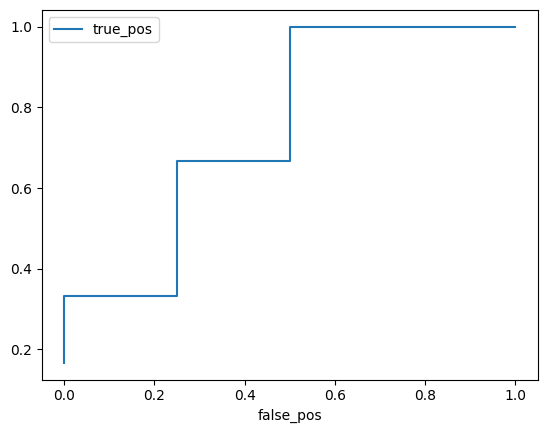
\includegraphics[width=0.8\textwidth]{hw3/1_5_a.png}\\
        \end{soln}
	
	\item (3pts) (Real-world open question) Suppose you want to choose a threshold parameter so that mails with confidence positives above the threshold can be classified as spam. Which value will you choose? Justify your answer based on the ROC curve.
	
	\begin{soln}  
            We do not want to mark any non-spam emails as spam, which means we want a false positive rate of 0. The confidence threshold which satisfies this property while having the highest true positive rate is 0.85
            \\This point on the ROC curve is the first kink in the curve starting from the bottom left of the graph.
        \end{soln}
\end{enumerate}

\item (8 pts) In this problem, we will walk through a single step of the gradient descent algorithm for logistic regression. As a reminder,
$$\hat{y} = f(x, \theta)$$
$$f(x;\theta) = \sigma(\theta^\top x)$$
$$\text{Cross entropy loss } L(\hat{y}, y) = -[y \log  \hat{y} + (1-y)\log(1-\hat{y})]$$
$$\text{The single update step } \theta^{t+1} = \theta^{t} - \eta \nabla_{\theta} L(f(x;\theta), y) $$



\begin{enumerate}
	\item (4 pts) Compute the first gradient $\nabla_{\theta} L(f(x;\theta), y)$.
	
	\begin{soln}
            We have that 
            \\$ \sigma'(z) = \sigma(z)(1-(\sigma(z)))$
            \\$ log'(x) = \frac{x'}{x}$
            
            $
            \\\nabla_{\theta} L(f(x;\theta), y) =
            \\\nabla_{\theta} -[y \log{(f(x;\theta))} + (1-y)\log{(1-f(x;\theta))}] = 
            \\\nabla_{\theta} -[y \log (\sigma(\theta^\top x)) + (1-y)\log(1-\sigma(\theta^\top x))] =
            \\ - [y \frac{\sigma(\theta^\top x) * (1-(\sigma(\theta^\top x)))}{\sigma(\theta^\top x)}*x + (1-y) \frac{-(\sigma(\theta^\top x) * (1-(\sigma(\theta^\top x))))}{1-\sigma(\theta^\top x)}*x] =
            \\ - x[ y (1-(\sigma(\theta^\top x))) + (1-y)(-\sigma(\theta^\top x)))] = 
            \\ - x[ y + (y)(-\sigma(\theta^\top x)) + (1-y)(-\sigma(\theta^\top x)))] =
            \\ - x[ y + (-\sigma(\theta^\top x))] =
            \\ x(\sigma(\theta^\top x) - y)
            $
        \end{soln}
	
	\item (4 pts)
 Now assume a two dimensional input. After including a bias parameter for the first dimension, we will have $\theta\in\mathbb{R}^3$.
$$ \text{Initial parameters : }  \theta^{0}=[0, 0, 0]$$
$$ \text{Learning rate }\eta=0.1$$
$$ \text{data example : } x=[1, 3, 2], y=1$$
Compute the updated parameter vector $\theta^{1}$ from the single update step.
	
	\begin{soln}
            $ \theta^{t+1} = \theta^{t} - \eta \nabla_{\theta} L(f(x;\theta), y)$, which means
            \\$\theta^{1} = \theta^{0} + \eta * x(\sigma(\theta^\top x) - y)
            \\ = [0,0,0] + 0.1 * [1,3,2] (\sigma([0,0,0] \dot [1,3,2]) - 1)
            \\ = [0,0,0] + 0.1 * [1,3,2] (0 - 1)
            \\ = [0,0,0] - 0.1 * [1,3,2]
            \\ = [-0.1, -0.3, -0.2]
            $
        \end{soln}
\end{enumerate}
\end{enumerate}

\section{Programming (50 pts)}
\begin{enumerate}
	\item (10 pts) Use the whole D2z.txt as training set.  Use Euclidean distance (i.e. $A=I$).
	Visualize the predictions of 1NN on a 2D grid $[-2:0.1:2]^2$.
	That is, you should produce test points whose first feature goes over $-2, -1.9, -1.8, \ldots, 1.9, 2$, so does the second feature independent of the first feature.
	You should overlay the training set in the plot, just make sure we can tell which points are training, which are grid.
	
	\begin{figure}[h]
		\centering
            Here is mine:
            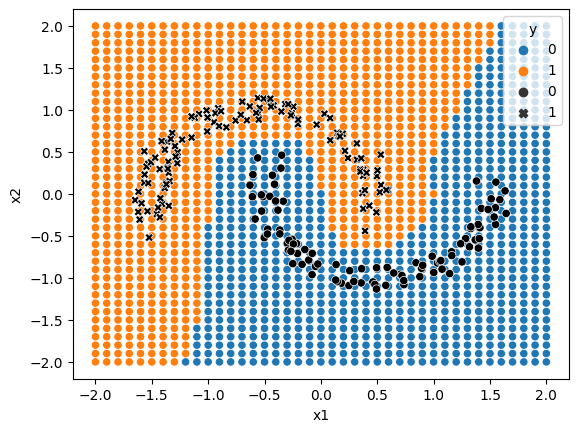
\includegraphics[width=0.8\textwidth]{hw3/2_1.png}\\
	\end{figure}
	
	\paragraph{Spam filter} Now, we will use 'emails.csv' as our dataset.
	
	\begin{itemize}
		\item Task: spam detection
		\item The number of rows: 5000
		\item The number of features: 3000 (Word frequency in each email)
		\item The label (y) column name: `Predictor'
		\item For a single training/test set split, use Email 1-4000 as the training set, Email 4001-5000 as the test set.
		\item For 5-fold cross validation, split dataset in the following way.
		\begin{itemize}
			\item Fold 1, test set: Email 1-1000, training set: the rest (Email 1001-5000)
			\item Fold 2, test set: Email 1000-2000, training set: the rest
			\item Fold 3, test set: Email 2000-3000, training set: the rest
			\item Fold 4, test set: Email 3000-4000, training set: the rest
			\item Fold 5, test set: Email 4000-5000, training set: the rest			
		\end{itemize}
	\end{itemize}
	
	\item (8 pts) Implement 1NN, Run 5-fold cross validation. Report accuracy, precision, and recall in each fold.
	
	\begin{soln}
            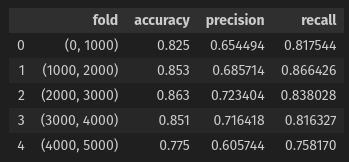
\includegraphics[width=0.4\textwidth]{hw3/2_2.png}\\
        \end{soln}
	
	\item (12 pts) Implement logistic regression (from scratch). Use gradient descent (refer to question 6 from part 1) to find the optimal parameters. You may need to tune your learning rate to find a good optimum. Run 5-fold cross validation. Report accuracy, precision, and recall in each fold.
	
	\begin{soln}  
            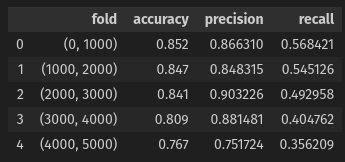
\includegraphics[width=6cm]{2_3.png}
        \end{soln}
	
	\item (10 pts) Run 5-fold cross validation with kNN varying k (k=1, 3, 5, 7, 10). Plot the average accuracy versus k, and list the average accuracy of each case. \\
	
	\begin{soln}
            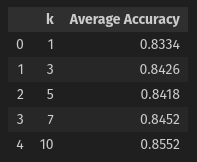
\includegraphics[width=4cm]{2_4_list.png}
    	\begin{figure}[h]
    		\centering
    		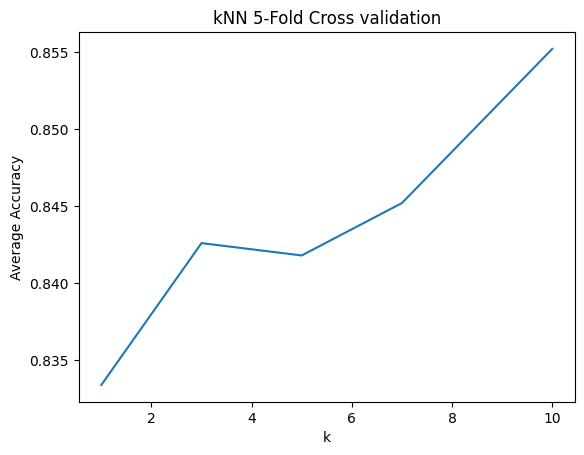
\includegraphics[width=10cm]{2_4.png}
    	\end{figure}
        \end{soln}
	
	\item (10 pts) Use a single training/test setting. Train kNN (k=5) and logistic regression on the training set, and draw ROC curves based on the test set. \\
	Expected figure looks like this.
	\begin{figure}[h]
		\centering
		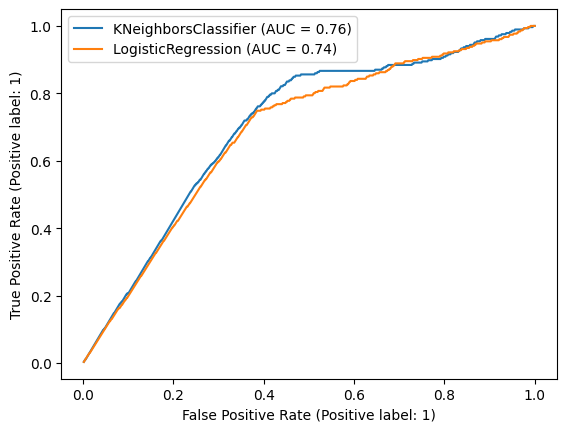
\includegraphics[width=8cm]{2_5.png}
	\end{figure}
	Note that the logistic regression results may differ.
	
	\begin{soln} 
            To be frank, I must have done something wrong but don't know what.
            Given that our algorithms should, in theory, be deterministic, may I ask for a kNN k=5 table of accuracies be provided to future students so they may know if their implementation is correct?
        \end{soln}
	
\end{enumerate}
\bibliographystyle{apalike}
\end{document}
